\bodychapter{INTRODUCTION}
\label{Intro}

Creating new types of visualization invariably requires programming.
Tools like Tableau~\cite{stolte2002polaris} create visualizations based on data and user input, but are limited to a relatively narrow selection of visualization types.
Many designers are trying their hands on visualization frameworks like D3~\cite{bostock2011d3}, but are not familiar enough with the programming concepts involved to be very effective.
At the same time, the theory of visual representation has not advanced much since the seminal work by Bertin~\cite{bertin1983semiology} and Mackinlay~\cite{Mackinlay1986}.
I believe that both problems can be solved by a fresh look at the nature of visual representation in visualization.

I propose a new model for the representation of data in information visualization: visualization primitives.
Like graphical primitives, visualization primitives are simple geometrical objects that can be combined into more complex ones.
The model provides easy access to the visual variables that each primitive object has (Figure~\ref{fig:primitive}).
The visual variables are similar to Bertin's retinal variables~\cite{bertin1983semiology}, and are customized per primitive to match the affordances of the primitive.
For example, a rectangle visualization primitive would provide access to height, width, left side, right side, top, bottom, horizontal midpoint, vertical midpoint, color, lineweight, etc.
In addition to just the graphical component, however, visualization primitives also connect to data and, in turn, produce output data.
In the rectangle example, all inputs have corresponding outputs, and outputs are calculated automatically given any input.
Automatic iteration through the data gives the user an experience of rapid visualization prototyping with immediate visual feedback.
By designing simple prototypes and applying data to them, users can quickly create many different visualizations in a very short time.

\begin{figure*}[t]
\centering
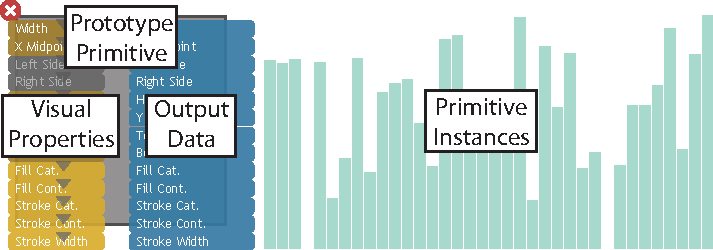
\includegraphics[width=\textwidth]{images/primitive.pdf}
\caption{A primitive rectangle in our implementation.}
\label{fig:primitive}
\end{figure*}

The goals of this work are as follows.
On the theory side, I want to develop a new model of visual data representation.
I believe that current models that are based on pipelines are too limited and do not adequately define the connection between visual appearance and data.
On the practical side, I believe that this model will translate into tools that better support creativity in the creation of data visualizations.
By producing interactions similar to design tools that work with graphical objects, visualization primitives will allow users to rapidly iterate with immediate feedback.
Immediate feedback and direct manipulation are key components of much creativity support software.